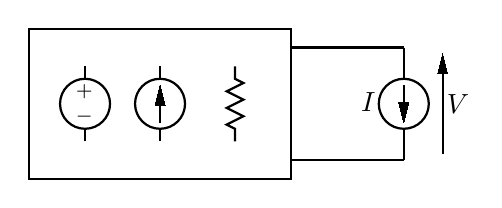
\begin{tikzpicture}[scale=2.54]
% dpic version 2020.06.01 option -g for TikZ and PGF 1.01
\ifx\dpiclw\undefined\newdimen\dpiclw\fi
\global\def\dpicdraw{\draw[line width=\dpiclw]}
\global\def\dpicstop{;}
\dpiclw=0.8bp
\dpiclw=0.8bp
\dpicdraw (0,0)
 --(0,0.0625)\dpicstop
\dpicdraw (0,0.1875) circle (0.049213in)\dpicstop
\draw (0,0.125) node{$_-$};
\draw (0,0.25) node{$_+$};
\dpicdraw (0,0.3125)
 --(0,0.375)\dpicstop
\dpicdraw (0.375,0)
 --(0.375,0.0625)\dpicstop
\dpicdraw (0.375,0.1875) circle (0.049213in)\dpicstop
\filldraw[line width=0bp](0.4,0.18125)
 --(0.375,0.28125)
 --(0.35,0.18125) --cycle\dpicstop
\dpicdraw (0.375,0.09375)
 --(0.375,0.258344)\dpicstop
\dpicdraw (0.375,0.3125)
 --(0.375,0.375)\dpicstop
\dpicdraw (0.75,0)
 --(0.75,0.0625)
 --(0.708333,0.083333)
 --(0.791667,0.125)
 --(0.708333,0.166667)
 --(0.791667,0.208333)
 --(0.708333,0.25)
 --(0.791667,0.291667)
 --(0.75,0.3125)
 --(0.75,0.375)\dpicstop
\dpicdraw (-0.28125,-0.1875) rectangle (1.03125,0.5625)\dpicstop
\dpicdraw (1.03125,0.46875)
 --(1.59375,0.46875)\dpicstop
\dpicdraw (1.59375,0.46875)
 --(1.59375,0.3125)\dpicstop
\dpicdraw (1.59375,0.1875) circle (0.049213in)\dpicstop
\filldraw[line width=0bp](1.56875,0.19375)
 --(1.59375,0.09375)
 --(1.61875,0.19375) --cycle\dpicstop
\dpicdraw (1.59375,0.28125)
 --(1.59375,0.116656)\dpicstop
\dpicdraw (1.59375,0.0625)
 --(1.59375,-0.09375)\dpicstop
\draw (1.46875,0.1875) node[left=-2bp]{$ I_{\opout}$};
\filldraw[line width=0bp](1.812935,0.3375)
 --(1.787935,0.4375)
 --(1.762935,0.3375) --cycle\dpicstop
\dpicdraw (1.787935,0.414594)
 --(1.787935,-0.0625)\dpicstop
\draw (1.787935,0.176047) node[right=-2bp]{$ V_{\opout}$};
\dpicdraw (1.59375,-0.09375)
 --(1.03125,-0.09375)\dpicstop
\end{tikzpicture}
